The data analysis of \textcite{Cheung2012CommunicationGaming}[572] revealed that players also rely on implicit awareness of each other’s gameplay status to adjust strategies silently. In their study, participants utilised verbal communication, virtual gestures and physical gestures.
To maintain mutual understanding and to form strategies based on common ground, players talk to each other directly \autocite{Cheung2012CommunicationGaming}[572]. As an example, a player could ask his teammate to split up, so they are able to attack an opponent from two different sides.

Another reason to talk to each other is the exchange for information, where the partner is in possession of information that needs to be shared. For example one player could have seen an enemy, but his teammate has no knowledge of this yet. As the writing of \textcite{Cheung2012CommunicationGaming}[573] says, a player can verbally announce their own status or actions that they thought would affect their partner. This could also effect the status of a player, for example the amount of health only the player itself is able to see.

\textcite{Cheung2012CommunicationGaming}[573] mentions that the announcing of points of interest, for example an spotted treasure, is often followed by or accompanied with a virtual gesture. They will point with their weapon onto objects they want to indicate, shoot at it or somehow use other possible gestures hey can use. They can even use they player characters position and running direction or rotation to indicate a direction.
In most situations virtual gestures provide a faster means to convey information than through verbal communication \autocite{Cheung2012CommunicationGaming}[573]. This virtual gestures are normally already understood by both players through previously gaming experiences, as they do not need to discuss the meaning of the gesture first \autocite{Cheung2012CommunicationGaming}[574].

Next to the communication channels \textcite{Cheung2012CommunicationGaming}[574] described, the awareness cues, which are categorised into central cues and peripheral cues, are also very important to maintain the awareness of the environment of each other in the game. 
\begin{itemize}
    \item Central Cues 
    
    Central cues are information the player is able to gain on his own through his own screen \autocite{Cheung2012CommunicationGaming}[574]. This indicates the current position, the direction and the remaining health of a player and each teammate. This also includes that a teammate is standing before an interact-able item.
    \item Peripheral Cues
    
    Peripheral cues are information, which are not restricted to functionality provided by the game \autocite{Cheung2012CommunicationGaming}[574]. Most of these cues are relating to co-location multiplayer games where a split-screen is used for example. A player could hear the other character screaming, which could indicate that the other player is in danger. Also a look onto the screen of a follow player counts to peripheral cues as stated by \textcite{Cheung2012CommunicationGaming}[574].
\end{itemize}

The third communication channel \textcite{Cheung2012CommunicationGaming}[572] described are physical gestures. Co-located players are able to point onto the screen with their hands, as well as other physical gestures such as waving. As this study not about co-location games, physical gestures are negligible, because it is not possible to use them in a network-based game per design.



\iffalse
----------------------
In online games, physical gestures cannot be used, because the players are not physically next
to each other. Virtual gestures can reach from using in-game avatar movement to using the
characters rotation and their utility (for example weapon) direction to point on certain things
(Cheung, Chang, and Scott 2012)[572]. Communication is not limited to direct methods of
transferring meaning (Toups et al. 2014)[258]. With changing environments, which includes
changing to or between gaming environments, communication needs to be dynamic. Language
evolves as individuals are exposed to new settings and need to convey novel meanings (Toups et
al. 2014)[258]. Toups et al. (2014)[259] classifies cooperative communication game mechanics
into three levels. Level one consists of environment-modifying, automated communication, immersive,
expressive, emergent and attention-focusing. With the modification of the environment
for example, players are able to permanently or semi-permanently change some components of
the game to convey information to other players (Toups et al. 2014)[259]. The computer games
Portal 21 and DOTA 22, in-game visual pointers enable player collaboration directly through
gameplay (Vaddi et al. 2016). Players are able to mark specific locations within the game,
where a visual attachment is placed. Next to a visual appearance, a notification sound to gain
the user’s attention is played. This example is one of indirect communication that can help
players to collaborate with each other.
----------------------
\fi




\subsection{Framework for cooperative communication game mechanics}
\label{section:Framework for cooperative communication game mechanics}

Communication is not limited to direct methods of transferring meaning \textcite{Toups2014ATheory}[258]. With changing environments, which includes
changing to or between gaming environments, communication needs to be dynamic. Language evolves as individuals are exposed to new settings and need to convey novel meanings \textcite{Toups2014ATheory}[258].
The language, as well as the communication channels, players are using are not totally equal to a dialogue between two persons. Games can give players individual customised tools, which improves the communication possibilities. 

\textcite{Toups2014ATheory}[258] used the virtual gestures \textcite{Cheung2012CommunicationGaming} described and created a framework of cooperative communication game mechanics to enable players to have rich game-centric communication.  
An investigation of different cooperative games, played by testers, showed communication mechanics the players were using. 

Figure \ref{fig:framework_cooperative_communication_mechanics} shows the three classifications which were used. 
Level one consists of environment-modifying, automated communication, immersive, expressive, emergent and attention-focusing. With the modification of the environment for example, players are able to permanently or semi-permanently change some components of the game to convey information to other players \textcite{Toups2014ATheory}[259]. 
Automated communication, expressive and attention focusing types are also having deeper classifications.
The computer games Portal 2\footnote{\url{https://store.steampowered.com/app/620/Portal_2/} - accessed on 30th January 2020} and DOTA 2\footnote{\url{https://store.steampowered.com/app/570/Dota_2/} - accessed on 30th January 2020}, in-game visual pointers enable player collaboration directly through gameplay \autocite{Vaddi2016Investigating2}[41]. 
Players are able to mark specific locations within the game,
where a visual attachment is placed. Next to a visual appearance, a notification sound is played to gain the user’s attention. This example is one of indirect communication that can help players to collaborate with each other.
In the following sub chapter, each game mechanic type is described further.

\begin{figure}
    \centering
    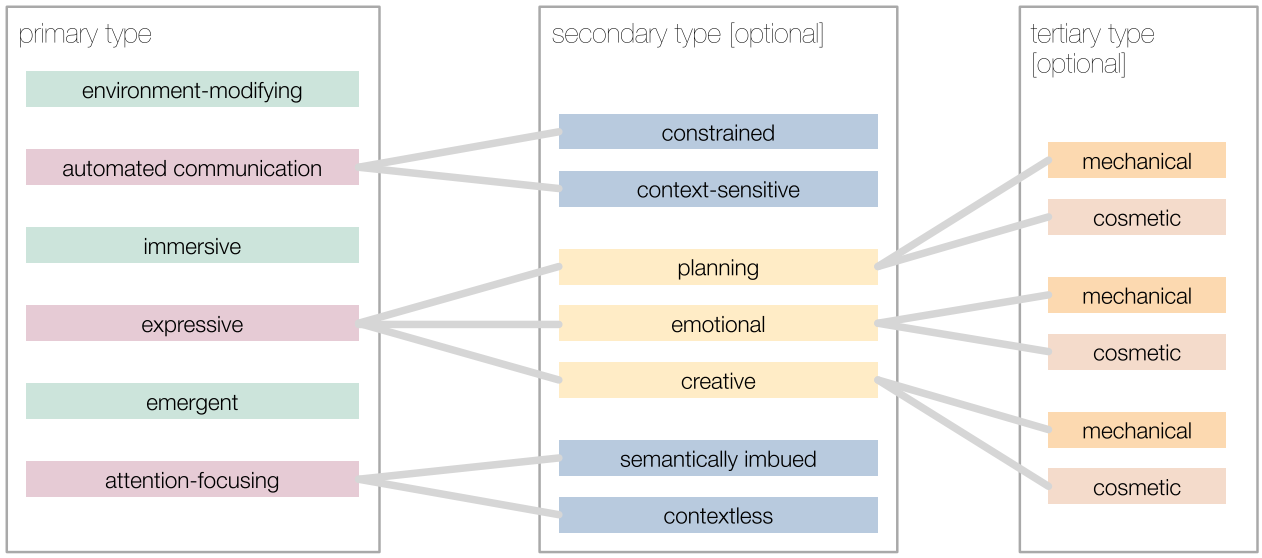
\includegraphics[scale=0.5]{images/framework_cooperative_communication_mechanics.png}
    \caption{\textcite{Toups2014ATheory}[259] divided their framework into up to three levels of classification for game mechanics.}
    \label{fig:framework_cooperative_communication_mechanics}
\end{figure}

\subsubsection{Environment-modifying}
\label{section:Environment-modifying}

Environment-modifying game mechanics allow players to permanently or semi-permanently change some component of the game world to convey information to other players \autocite{Toups2014ATheory}[259].
This reaches from creating signs for an indicated path, other players or the player themselves can follow, to the possibility to create lore created by players, which can merge with the game world. The investigation of \textcite{Toups2014ATheory}[260] showed, that although they can be used to grief or troll players, there are interesting environment-modifying mechanics.
For future help, they could be used to provide information to future players to guide them trough a labyrinth.

Signposts are one of \textcite{Toups2014ATheory}[260] exemplar mechanics, which generally involves players to take a break from other gameplay to interact with a messaging sub-system. Other players on the other hand have to pause their current goal too, to read the sign. This mechanics also do not have to be synchronous.
Players do not need another player to be online. The sign could be placed one week before a player finds it and the message can still be passed to the player. \textcite{Cheung2012CommunicationGaming}[260] mentions the signpost mechanics in \textit{Dark Souls} and \textit{Dark Souls II}, where players can leave messages on the ground, as well as \textit{Minecraft}, which allows players to create signs with short text messages. These signposts are permanently placed, as long as a player does not remove it. As Minecraft allowed players to create buildings, bridges and so on with block-sized voxels, players are also able to create allow-like shapes, which are also count as an environment-modifying mechanic.


\subsubsection{Automated communication}
\label{section:Automated communication}

Automated communication is divided into constrained and context sensitive mechanics.
Constrained automated communication mechanics take the form of pre-defined announcements or responses that the player invokes to explicitly indiate somthing to teammates \autocite{Toups2014ATheory}[260].

"Message Macros" allow the player to efficiently select from a limited set of pre-generated messages and share them with teammates. Instead of typing whole messages into the chat, a player can send messages by a combination of buttons.
The Games Tribes\footnote{\url{https://web.archive.org/web/20151028195605/http://www.hirezstudios.com/tribesascend/home} - accessed on 13th June 2020}, a fast team-based first person shooter, as well as Smite\footnote{\url{https://www.smitegame.com} - accessed on 13th June 2020}, a 5 VS 5 player strategy game, implemented a Voice Guided System (VGS). To warn teammates about a missing enemy in the left game-area, a player in Smite can type \textit{VF1}\footnote{\url{https://smite.gamepedia.com/VGS_Cheat_Sheet} - accessed on 13th June 2020}. This sends the message "Enemy missing left!" to the text-chat and plays a voice-recorded audio feedback to all team members.
Another (corner) case is the possibility to sing in \textit{Journey\footnote{\url{https://thatgamecompany.com/journey/} - accessed on 13th June 2020}}. It is the only communication mechanic and allows the player to interact with the environment and allows other players to locate the game character. Additionally it is counted to being an emergent communication mechanic \autocite{Toups2014ATheory}[261].


Context-Sensitive automated communication mechanics rely on state to parameterize a communication to teammates \autocite{Toups2014ATheory}[261]. It simplifies the exchanging of information between players by allowing players to share information, which seems to be understood by the game itself.
Contextual macros are sending pre-defined information to other players, regarding the currently selected item. In \textit{Diablo III\footnote{\url{https://eu.diablo3.com/de/} - accessed on 13th June 2020}}, a player is able to send the description of a piece of treasure to allies, which normally is only visible to the player who is carrying the item \autocite{Toups2014ATheory}[261].

Context-sensitive automated communication however is more limited, because they this mechanics need to be well planned by the designer. They are only usable in A specific context and may be not usable for the player, when the function in an unfamiliar way \autocite{Toups2014ATheory}[261]. 


\subsubsection{Immersive}
\label{section:Immersive}

Immersive communication mechanics invite teammates to join a shared experience, rather than directing other players towards a specific game-winning behaviour \autocite{Toups2014ATheory}[261].
Immersive mechanics are connected to the game-character and improves the experience within the game. The perfect example for immersive mechanics are character emotes. The player character can act on their own by showing a laughing, dancing or waving animation. But also interactions such as high-fives or playing rock-paper-scissors in \textit{Portal 2\footnote{\url{https://store.steampowered.com/app/620/Portal_2/} - accessed on 30th January 2020}} between multiple players are possible.

\subsubsection{Expressive}
\label{section:Expressive}
 Expressive communication mechanics support players in sharing information about themselves, as well as planning and sharing emotions or to be creative \autocite{Toups2014ATheory}[261]. They are more deeply classified by whether they enact state change on the game or if they are only cosmetic \autocite{Toups2014ATheory}[261].


Expressive planning communication mechanics are used to direct teammates to future gameplay. This includes situational holding mechanics, like holding a weapon. In open-world survival games like \textit{Rust\footnote{\url{https://rust.facepunch.com/} - accessed on 13th June 2020}} or DayZ\footnote{\url{https://dayz.com/} - accessed on 13th June 2020} showing a weapon can indicate that the player is ready for combat and running around without weapons can indicate peace. As \textcite{Toups2014ATheory}[262] notices, this behaviour works because it gives a player a clear disadvantage when violence erupts. Therefore the current equipment is connected to the trust players have towards their teammates and opponents.


Expressive emotional mechanics gives the player the possibility to express themselves to their team. \textcite{Toups2014ATheory}[262] said that expressing their emotions via communication mechanics, positive emotions could cascade through the team when they are shared with them. Gesture mechanics are an example, as an character animation like a thumb-up or trying to hug another player can indicate happy emotions. This animations are often either triggered by writing a text-command into the chat or by any kind of button combination. In \textit{Portal 2} it is possible for a player to give their teammates a high-five, to cheer a successful action together. As these animations have to be pre-defined, players are limited to a selection of gestures provided, but do not have to articulate how they feel in words \autocite{Toups2014ATheory}[262].

\textcite{Toups2014ATheory} do not give any example for creative expressive communication mechanics. Being able to draw images onto walls could be a combination between environment-modifying and creative expressive mechanic, as players are able to express themselves through a cosmetic way to communicate with other players.


\subsubsection{Emergent}
\label{section:Emergent}

Emergent cooperative communication mechanics seem to be different from other mechanics, because they are not necessary implemented to give players the opportunity to communicate with it. They communication with this mechanics exists between certain communities and have to be learned \autocite{Toups2014ATheory}[262]. One example many games have implemented is the possibility to jump, which in the first place is implemented because of movement reasons. However, jumping without any reason can have a semantic meaning, which can mean nearly everything, starting from "Pay attention to me" to "I am impatient" \autocite{Toups2014ATheory}[262]. 
The player community of Smite developed the act of jumping around together with enemy players before the match started as a good sign of will and to wish every player luck and fun. This behaviour is not intended by the game designers and new players do not know about it, unless they read about it or it is explained by another player.

\subsubsection{Attention-focusing}
\label{section:Attention-focusing}

Attention-focusing game mechanics provides players the possibility to gain attention, point onto objects other players should focus on or to give commands, teammates should follow. Giving teammates a description where they need to look at can be more difficult than pointing at it. There are two different types of attention-focusing mechanics, which are either bound to a specific context ore are context-less \autocite{Toups2014ATheory}[262].


A well known communication mechanic is the ping mechanic. Players can click onto the map to create a icon in the virtual game space. Some games combine these with an sound effect to gain the attention of the player, who may look at a different part of the environment.
The most prominent games which provide pings a strategy games, where the position can of characters can have an important value. In strategy games from the \textit{Starcraft\footnote{\url{https://starcraft2.com/de-de/} - accessed on 13th June 2020}} or \textit{Warcraft\footnote{\url{https://playwarcraft3.com/de-de/} - accessed on 13th June 2020}} series, players can ping on the environment or mini-map, which is displayed on their and their allies screen \autocite{Toups2014ATheory}[]263]. The ping itself however has no greater meaning and only highlights a certain position. The purpose of the ping itself needs to be communicated or is understood by all parties through previous experiences.


Attention focusing communication game mechanics can have a semantically imbued meaning, which provides information or carry along commands. \autocite{Toups2014ATheory}[263].
In \textit{League of Legends\footnote{\url{https://leagueoflegends.com/} - accessed on 13th June 2020}} pings can be context-less, but can also be "Augmented environment Pings". The game contains structures such as allied and enemy towers. Clicking on different parts of the game words creates different pings. By creating a ping at the enemy tower, instead of a normal ping with a blue dot, a ping with an red exclamation point appears above the target \autocite{Toups2014ATheory}[263]. Next to the function of pointing at different positions, these augmented pings can tell teammates to defend or attack a certain character or structure.

In \textit{Portal 2} it is possible to choose between different types of pings. Next to a simple "look at"-ping, there are also pings with different icons to indicate that at this position a partner should create a portal. For time-based interactions there is also a countdown-ping, which can improve time-based actions a lot, even with out verbally communicating with each other.